\documentclass[12pt,a4paper]{journal}
\usepackage[margin=1in]{geometry}

\usepackage[utf8]{inputenc}
\usepackage[T1]{fontenc}
\usepackage{indentfirst}
\usepackage{amsmath}
\usepackage{amsfonts}
\usepackage{amssymb}
\usepackage{caption}
\usepackage{subcaption}
\usepackage{graphicx}
\usepackage{siunitx}
\sisetup{range-phrase=--, range-units=single}

\graphicspath{{img/}}
\usepackage[numbers, square]{natbib}


\begin{document}

\subsection{Physiology of the retina}

Images to include:
\begin{itemize}
\item diagram of the organization of the eye (overall structure)
\item diagram/picture of the organization of the retinal layers
\item images of healthy retinal scans (structural/angiogram)
\end{itemize}


\subsubsection{In health}

\begin{itemize}
\item organization of the eye: iris/lens..., vitreous, retina, choroid, sclera
\item organization of the retina: optic nerve head, macula, fovea, the difference layers of cells
\item how each layer is attached to each other
\item how incoming light is processed: travels through the retina, captured by photoreceptors, transformed in biochemical signal, transform in elecrtical signal, sent through the optic nerve to the brain
\item the vasculature in the retina and the choroid (add where it comes from, i.e., ophthalmic artery?)
\item ajouter des images de healthy/diseased retinae OCTA/FA and OCT
\item role du RPE
\end{itemize}

\large\textbf{organization of the eye: iris/lens..., vitreous, retina, choroid, sclera}

The retina is a layer of tissue, aproximately \SI{0.5}{\mm} thick, that lines the back of the eye.
The retinal inner surface is attached to the vitreous body, the clear gel that separates the lens and the retina, while its outer surface is attached to Bruch's membrane, see Figure~\ref{fig:architecture-eye}.
When looking at a cross section of the retina as shown in Figure~\ref{fig:architecture-eye}, eight layers can be identified, the innermost (closest to the vitreous) being the optic nerve fibers layer and the outermost the retinal pigmented epithelium (RPE).\\
In the centre of the retina is a oval-shaped pigmented area called the macula.
The macula is about \SI{5}{\mm} wide and is responsible for the highly detailed, central vision thanks to its high concentration of photoreceptor cells, namely rods and cones.
In particular, cones are highly concentrated in the centre of the macula, in a pit approximately \SI{1.5}{\mm} wide named the fovea.
The optic nerve fibers layer 

\begin{figure}[h]
  \centering
  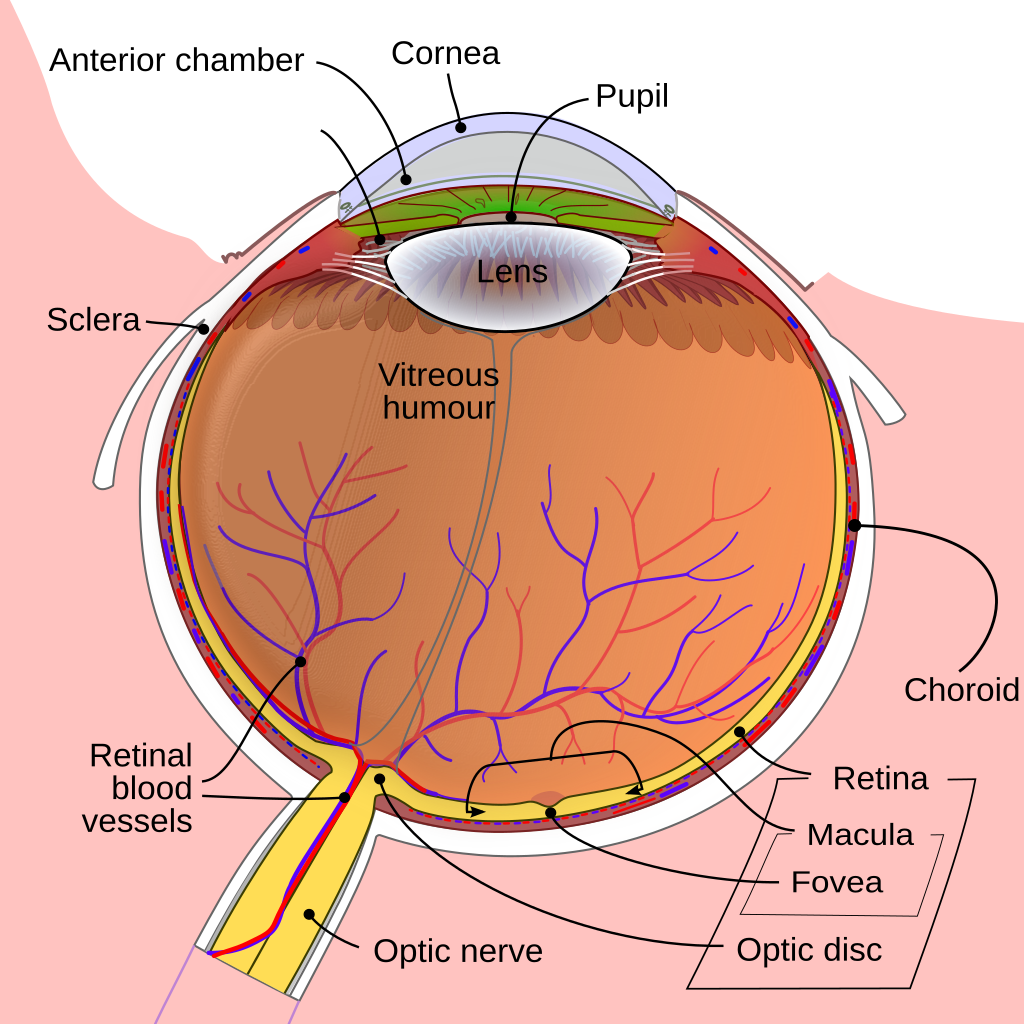
\includegraphics[width=0.45\textwidth, height=7cm]{ArchitectureEye} % From Wikipedia retina
  \hfill
  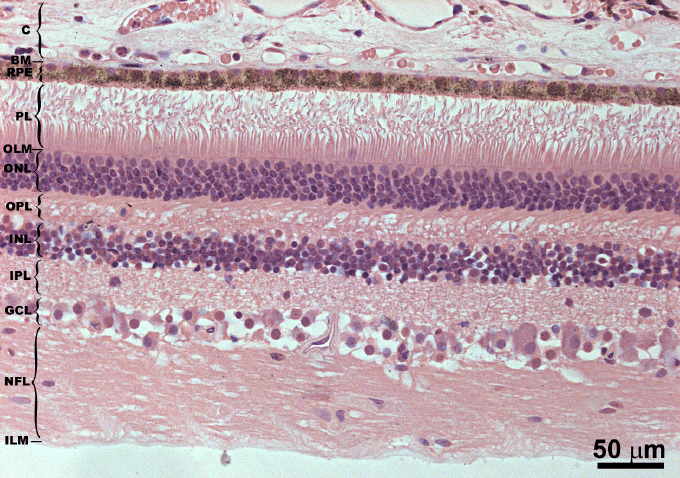
\includegraphics[width=0.45\textwidth, height=7cm]{RetinaHistology}
  \caption{General architecture of the eye and the retina. This is for illustration, taken from Wikipedia and 'Glia and blood retinal barrier: effects of ocular hypertension' and rights need to be checked/the pics need to be eddited.}
  \label{fig:architecture-eye}
\end{figure}
\subsubsection{In disease}

\begin{itemize}
\item degradation of the blood supply chain (rarefaction des vaisseaux sanguins dans la retine (e.g. en cas de diabete) et le choriocapillaris (e.g. AMD)
\item augmentation de la pression occulaire (IOP) in, e.g., glaucoma
\item epaississement de la membrane de Bruch avec l'age et peut-etre AMD?
\item formation de drusen in AMD et avec l'age et le risque de detachement de la retine ou du RPE
\item neovascularisation et leakages
\end{itemize}

% \begin{spacing}{0.0}
\bibliographystyle{abbrvnat} % {ksfh_nat}
{\normalsize \bibliography{section_2}}
% \end{spacing}

\end{document}
